\section{Adapter Pattern}

Adapter pattern works as a bridge between two incompatible interfaces. This type of design pattern comes under structural pattern as this pattern combines the capability of two independent interfaces.

This pattern involves a single class which is responsible to join functionalities of independent or incompatible interfaces. A real life example could be a case of card reader which acts as an adapter between memory card and a laptop. You plugin the memory card into card reader and card reader into the laptop so that memory card can be read via laptop.

We are demonstrating use of Adapter pattern via following example in which an audio player device can play mp3 files only and wants to use an advanced audio player capable of playing vlc and mp4 files. 

\subsection{Implementation}

We have a MediaPlayer interface and a concrete class AudioPlayer implementing the MediaPlayer interface. AudioPlayer can play mp3 format audio files by default.

We are having another interface AdvancedMediaPlayer and concrete classes implementing the AdvancedMediaPlayer interface. These classes can play vlc and mp4 format files.

We want to make AudioPlayer to play other formats as well. To attain this, we have created an adapter class MediaAdapter which implements the MediaPlayer interface and uses AdvancedMediaPlayer objects to play the required format.

AudioPlayer uses the adapter class MediaAdapter passing it the desired audio type without knowing the actual class which can play the desired format. AdapterPatternDemo, our demo class will use AudioPlayer class to play various formats.

\subsection{Class Diagram}

\begin{figure}[h]
\centering
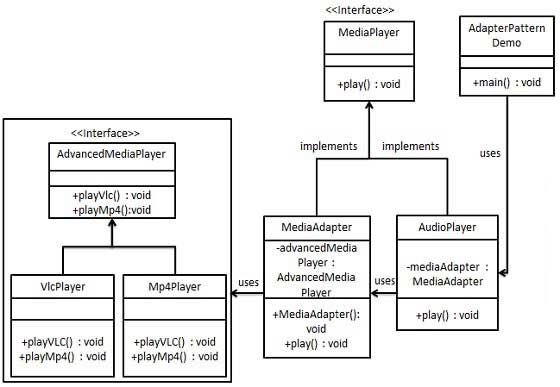
\includegraphics[scale=0.7]{adapter}
\caption{Class Diagram of Adapter Pattern}
\end{figure}

\newpage
\subsection{Source Code (Java)}

\subsubsection{MediaPlayer Interface}

\begin{minted}{java}
public interface MediaPlayer {
   public void play(String audioType, String fileName);
}
\end{minted}

\subsubsection{AdvancedMediaPlayer Interface}

\begin{minted}{java}
public interface AdvancedMediaPlayer {	
   public void playVlc(String fileName);
   public void playMp4(String fileName);
}
\end{minted}

\subsubsection{AdvancedMediaPlayer Class}

\begin{minted}{java}
public class VlcPlayer implements AdvancedMediaPlayer{
   @Override
   public void playVlc(String fileName) {
      System.out.println("Playing vlc file. Name: "+ fileName);		
   }

   @Override
   public void playMp4(String fileName) {
      //do nothing
   }
}
\end{minted}

\subsubsection{Mp4Player Class}

\begin{minted}{java}
public class Mp4Player implements AdvancedMediaPlayer{

   @Override
   public void playVlc(String fileName) {
      //do nothing
   }

   @Override
   public void playMp4(String fileName) {
      System.out.println("Playing mp4 file. Name: "+ fileName);		
   }
}
\end{minted}

\subsubsection{MediaAdapter Class}

\begin{minted}{java}
public class MediaAdapter implements MediaPlayer {

   AdvancedMediaPlayer advancedMusicPlayer;

   public MediaAdapter(String audioType){
   
      if(audioType.equalsIgnoreCase("vlc") ){
         advancedMusicPlayer = new VlcPlayer();			
         
      }else if (audioType.equalsIgnoreCase("mp4")){
         advancedMusicPlayer = new Mp4Player();
      }	
   }

   @Override
   public void play(String audioType, String fileName) {
   
      if(audioType.equalsIgnoreCase("vlc")){
         advancedMusicPlayer.playVlc(fileName);
      }
      else if(audioType.equalsIgnoreCase("mp4")){
         advancedMusicPlayer.playMp4(fileName);
      }
   }
}
\end{minted}

\subsubsection{AudioPlayer Class}

\begin{minted}{java}
public class AudioPlayer implements MediaPlayer {
   MediaAdapter mediaAdapter; 

   @Override
   public void play(String audioType, String fileName) {		

      //inbuilt support to play mp3 music files
      if(audioType.equalsIgnoreCase("mp3")){
         System.out.println("Playing mp3 file. Name: " + fileName);			
      } 
      
      //mediaAdapter is providing support to play other file formats
      else if(audioType.equalsIgnoreCase("vlc") || audioType.equalsIgnoreCase("mp4")){
         mediaAdapter = new MediaAdapter(audioType);
         mediaAdapter.play(audioType, fileName);
      }
      
      else{
         System.out.println("Invalid media. " + audioType + " format not supported");
      }
   }   
}
\end{minted}

\subsubsection{Driver Class}

\begin{minted}{java}
public class AdapterPatternDemo {
   public static void main(String[] args) {
      AudioPlayer audioPlayer = new AudioPlayer();

      audioPlayer.play("mp3", "beyond the horizon.mp3");
      audioPlayer.play("mp4", "alone.mp4");
      audioPlayer.play("vlc", "far far away.vlc");
      audioPlayer.play("avi", "mind me.avi");
   }
}
\end{minted}

\subsection{Output}

\begin{minted}{text}
Playing mp3 file. Name: beyond the horizon.mp3
Playing mp4 file. Name: alone.mp4
Playing vlc file. Name: far far away.vlc
Invalid media. avi format not supported
\end{minted}
